% Intended LaTeX compiler: pdflatex
\documentclass{scrartcl}
		\usepackage[utf8]{inputenc}
		\usepackage[dvipdfmx]{graphicx}
		\usepackage[dvipdfmx]{color}
		\usepackage[backend=biber,bibencoding=utf8]{biblatex}
		\usepackage{url}
		\usepackage{indentfirst}
		\usepackage[normalem]{ulem}
		\usepackage[dvipdfmx]{hyperref}
		\usepackage{fancyvrb}
                \usepackage{minted}
		\usepackage[top=25truemm,bottom=25truemm,left=25truemm,right=25truemm]{geometry}
\author{筑波大学情報科学類2年 江畑 拓哉 (201611350)}
\date{}
\title{論理回路実験レポート}
\begin{document}

\maketitle
\section{右方向シフトレジスタのネットリスト/回路図}
\label{sec:orgf6d78de}
使用したもの(実験に用いた)\\
\begin{itemize}
\item 74HC74 * 2 ( U1 ,U2 )\\
\item データ出力端子D0 ( ICT\_D.0 )\\
\item データ入力端子 * 5   ( ICT\_I.0, 1, 2, 3, 4, 5 )\\
\item パルス出力端子 ( ICT\_D.A )\\
\item 電源/GND ( ICT\_+5V ICT\_GND )\\
\item ジャンパ線 数十本\\
\item 単芯 数本\\
\end{itemize}
\subsection{ネットリスト}
\label{sec:org1a4bc2c}

\begin{minted}[frame=lines,linenos=true,obeytabs,tabsize=4]{text}
N0001: U1.1 U1.4 U1.13 U1.10
       U2.1 U2.4 U2.13 U2.10
       ICT_+5V
N0002: U1.2 ICT_D.0 ICT_I.4
N0003: U1.5 U1.12   ICT_I.3 
N0004: U1.9 U2.2    ICT_I.2
N0005: U2.5 U2.12   ICT_I.1
N0006: U2.9 ICT_I.0
N0007: U1.3 U1.11 
       U2.3 U2.11 
       ICT_D.A
\end{minted}
\subsection{回路図のコピー}
\label{sec:org26de43e}
\begin{center}
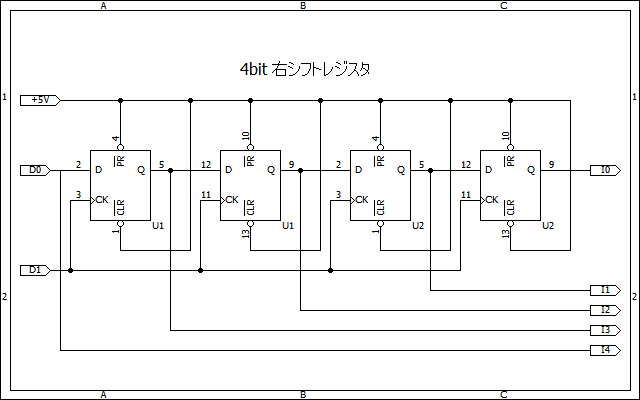
\includegraphics[width=15cm]{./logic.png}
\end{center}
\section{Clockにデータスイッチを使っ場合の動作の観測とその考察}
\label{sec:org3f637d9}
 Clockをつなぐ端子をパルス出力端子から、データ出力端子に変えた際の違いを観測したところ、見受けられた違いは以下のとおりであった。\\
\begin{itemize}
\item 順番ではなく一気にカウントが進んだ。\\
\item スイッチを動かしても反応しないことがあった、\\
\item 途中でリセットされた。\\
\end{itemize}
 また、これらの問題が起こった場合の共通点としてデータ出力に用いたスイッチを高速に動作させたことが挙げられる。残念ながら、ゆっくりとスイッチを操作した場合ではパルススイッチとほとんど変わらない動作をした。\\
\subsection{本来起こってほしい動作}
\label{sec:orge86bb06}
以下に本来起こってほしい動作のタイミングチャートを示す。\\
\begin{center}
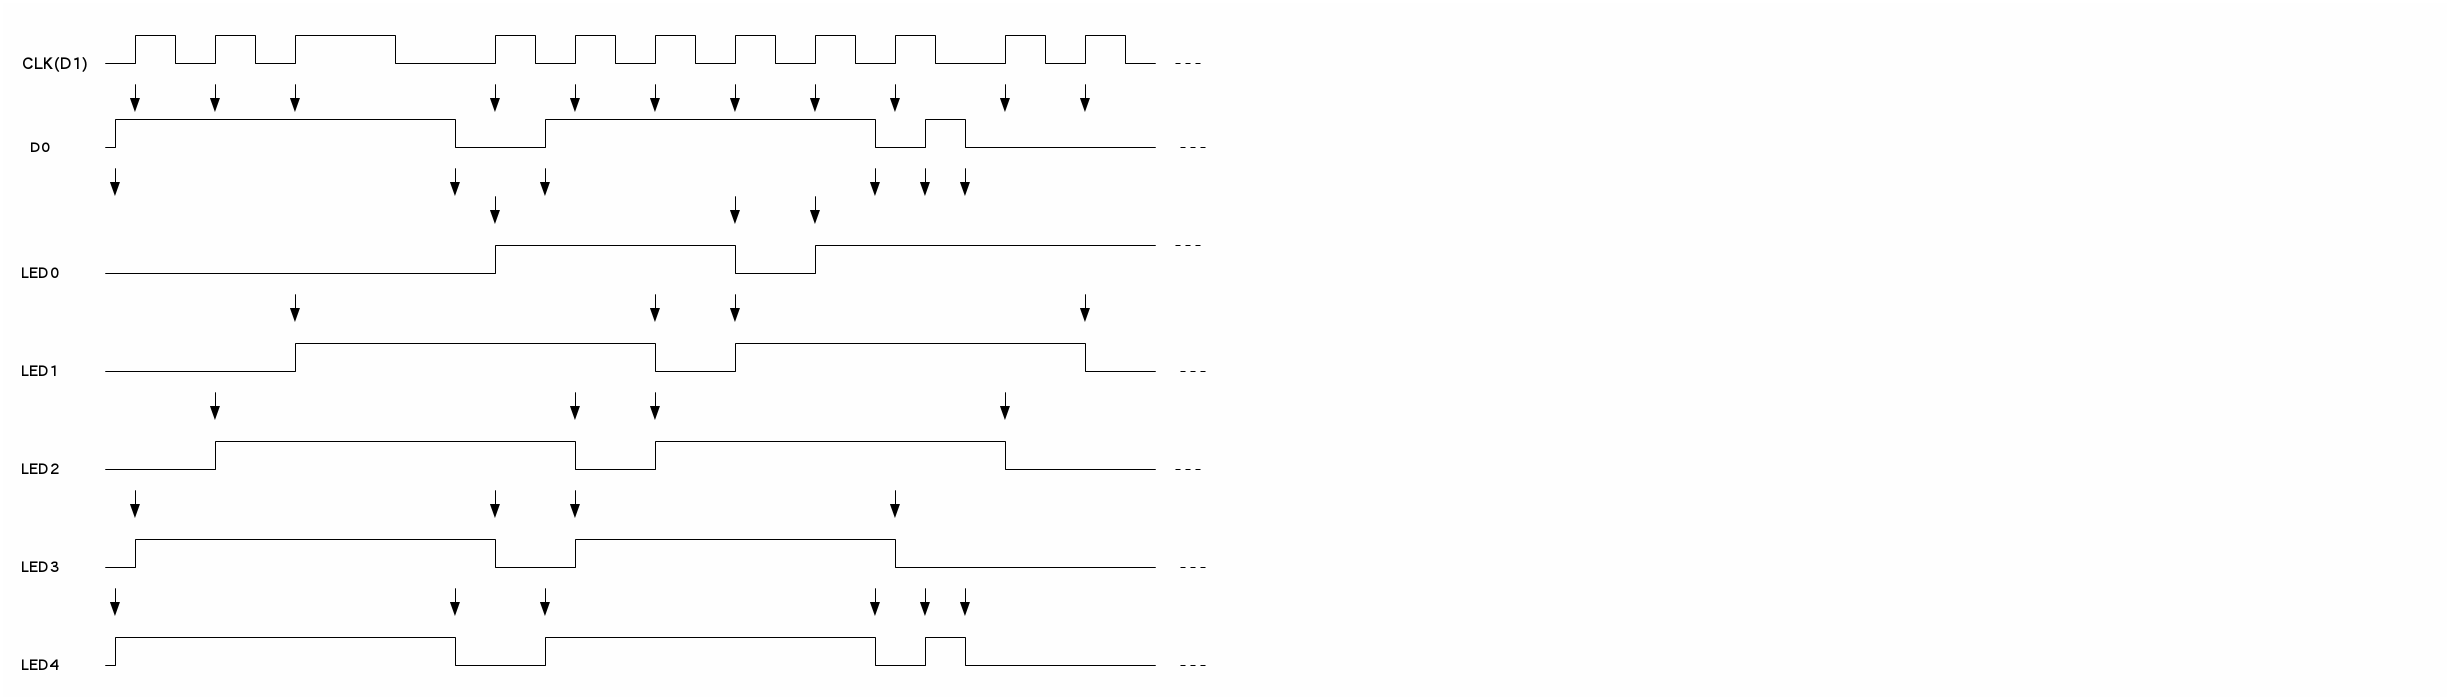
\includegraphics[width=1.5\linewidth]{flowchart1.png}
\end{center}


\subsection{起きた問題}
\label{sec:orge4a0a65}
起きた問題についてのタイミングチャートを順に示す。\\
\begin{center}
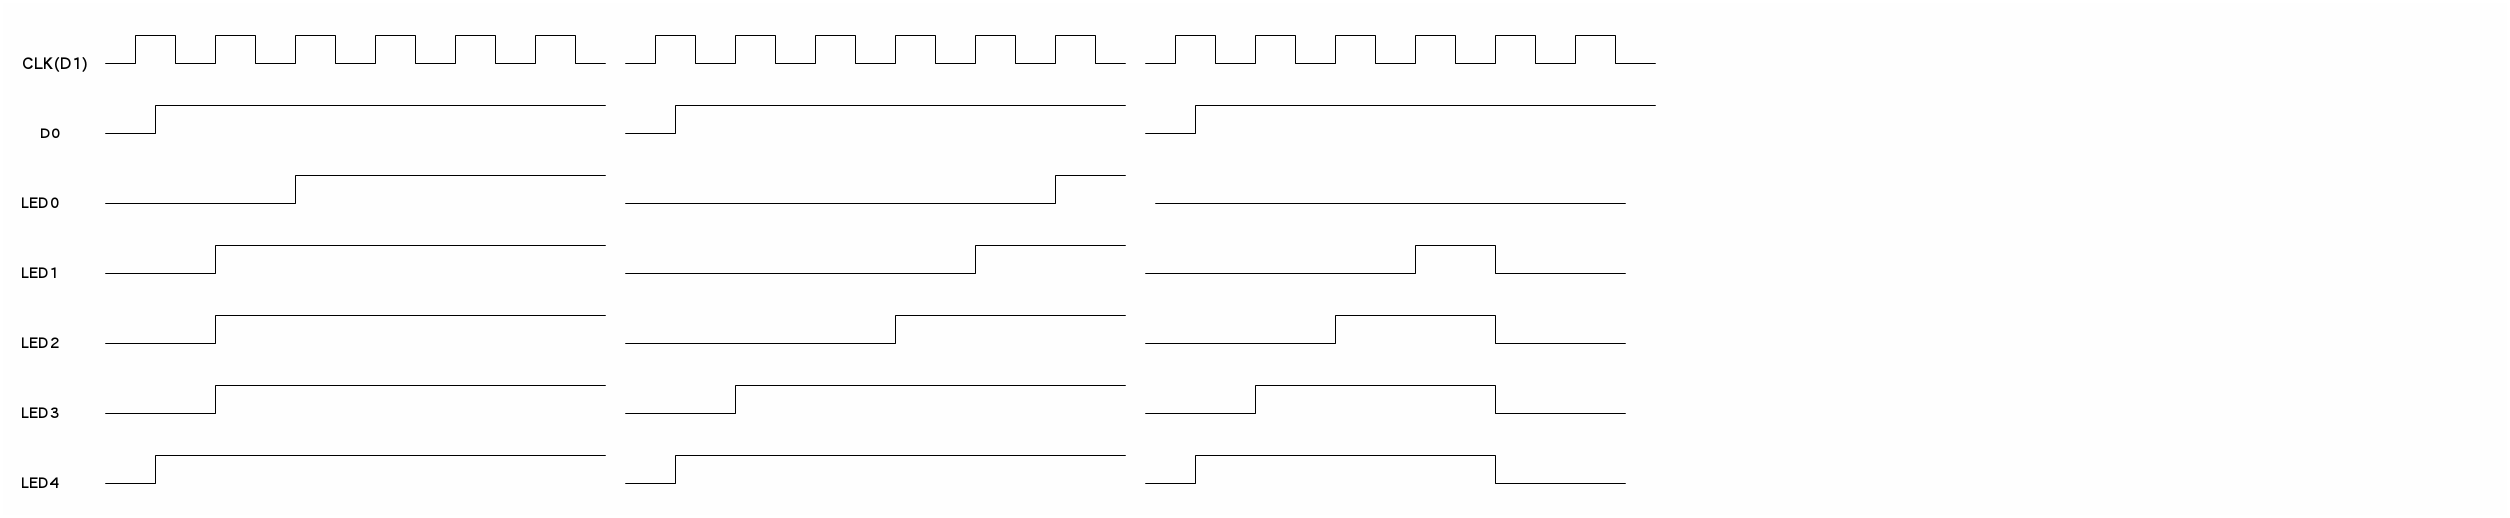
\includegraphics[width=1.5\linewidth]{flowchart2.png}
\end{center}


\subsection{原因と考えられるもの}
\label{sec:org494d8f3}

    原因としてまず考えられるものとして、チャタリングによる値の不確実さが挙げられる。言うまでもないがチャタリングとは入力の変化に値が不安定になってしまうことで、その時間中は入力の値は不定とされる。つまり、早い時間でスイッチを高速に動作させるとチャタリングによる不安定さも相まって信号が正しく伝わらなくなる可能性が出てくるのだ。この動作の不具合は人から見てスイッチの切り替えが明白であるデータスイッチにおいてわかりやすい違和感として感じられるだろう。\\
  また、同様にD-FFの構造的な問題も考えられるだろう。\\
    更には、ジャンパ線の多様による回路の煩雑化もこの不安定さに一役買っていると考えられる。この実験では、単芯と長いジャンパ線を用いて配線を行うが、私の場合回路の最適化を怠っており、長いジャンパ線がICトレーナーを覆っている状態になっていた。このような無駄の多い配線は、それだけ電気信号の伝達に遅れが出ることは明白である。\\
  また、使用している機材そのものの問題も考えられる。例えばブレットボードの漏電、ジャンパ線の劣化(途中の断線)が考えられる。\\
  \\

\subsection{対策}
\label{sec:org63fbeee}

 対策としては、チャタリング除去機能のあるICを使うようにすることや、配線を最適化すること、配線に於いてできる限りテスターを用いて確認をすること、極端に高速で動かさないことを挙げることができるだろう。\\
 具体的には、NOTゲートで使用している74HC04を74HC14に変えること、できる限りのジャンパ線から単芯への移行、小さな配線のグループ単位でのテスト、そして慌てずにテストを行える余裕を持つことが考えられる。\\
\subsection{批判}
 この課題では問題の起きにくい、つまり今までの考察より考えれば、最適化された回路を制作した学生には難しかったのではないだろうか。もっともそれだけ技術がある学生はより繊細な問題を発見するだろうとは考えられる。\\
 一部の学生間ではより細かい繊細な問題を確認していたようだが、初学者でこの分野における詳しい研究を積んでいない自分としてはもう少し参考文献をいただきたいと考えている。
\subsection{参考文献}
 昨年度の論理回路の指定教科書である「だれにもわかるディジタル回路」を用いた他、教員のアドバイスを参考にした。
\end{document}
